\documentclass[11pt,a4paper]{article}
\usepackage[utf8]{inputenc}
\usepackage{booktabs}
\usepackage{graphicx}
\usepackage{amsmath}
\usepackage{hyperref}
\usepackage[margin=1in]{geometry}
\usepackage{float}

\title{Qwen2.5-VL-3B: Zero-Shot Robust vs Blended Prompting \\ on CIFAR-10 Corruptions}
\author{VizInt Experiment}
\date{\today}

\begin{document}
\maketitle

\begin{abstract}
We evaluate Qwen/Qwen2.5-VL-3B-Instruct (4-bit quantized) as a zero-shot classifier on CIFAR-10 with image corruptions. Two prompting strategies are compared: \textbf{Robust} (classify only) and \textbf{Blended} (identify corruption then classify). Evaluated on 1000 images per condition.
\end{abstract}

\section{Method}
The Robust prompt asks the VLM to classify into CIFAR-10 categories via JSON output. The Blended prompt additionally asks the model to identify the corruption type (none, gaussian\_noise, rotation, affine) before classifying, mirroring how auxiliary transform prediction heads improve traditional models.

\section{Results}
\begin{table}[H]
\centering
\caption{Classification accuracy at various corruption severities.}
\begin{tabular}{lccccccc}
\toprule
\textbf{Model} & \textbf{Clean} & \textbf{S=0.25} & \textbf{S=0.5} & \textbf{S=0.75} & \textbf{S=1.0} & \textbf{Avg Drop} & \textbf{OOD} \\
\midrule
Qwen2.5-VL-3B Robust & 0.8270 & 0.5860 & 0.5090 & 0.4690 & 0.4660 & 0.3195 & 0.3890 \\
Qwen2.5-VL-3B Blended & 0.7810 & 0.4970 & 0.4480 & 0.4400 & 0.4130 & 0.3315 & 0.3390 \\
\bottomrule
\end{tabular}
\end{table}

\begin{table}[H]
\centering
\caption{Per-transform accuracy at S=1.0.}
\begin{tabular}{lccc}
\toprule
\textbf{Model} & \textbf{Gaussian Noise} & \textbf{Rotation} & \textbf{Affine} \\
\midrule
Qwen2.5-VL-3B Robust & 0.1119 & 0.2996 & 0.6506 \\
Qwen2.5-VL-3B Blended & 0.0702 & 0.2622 & 0.5510 \\
\bottomrule
\end{tabular}
\end{table}

\begin{figure}[H]
\centering
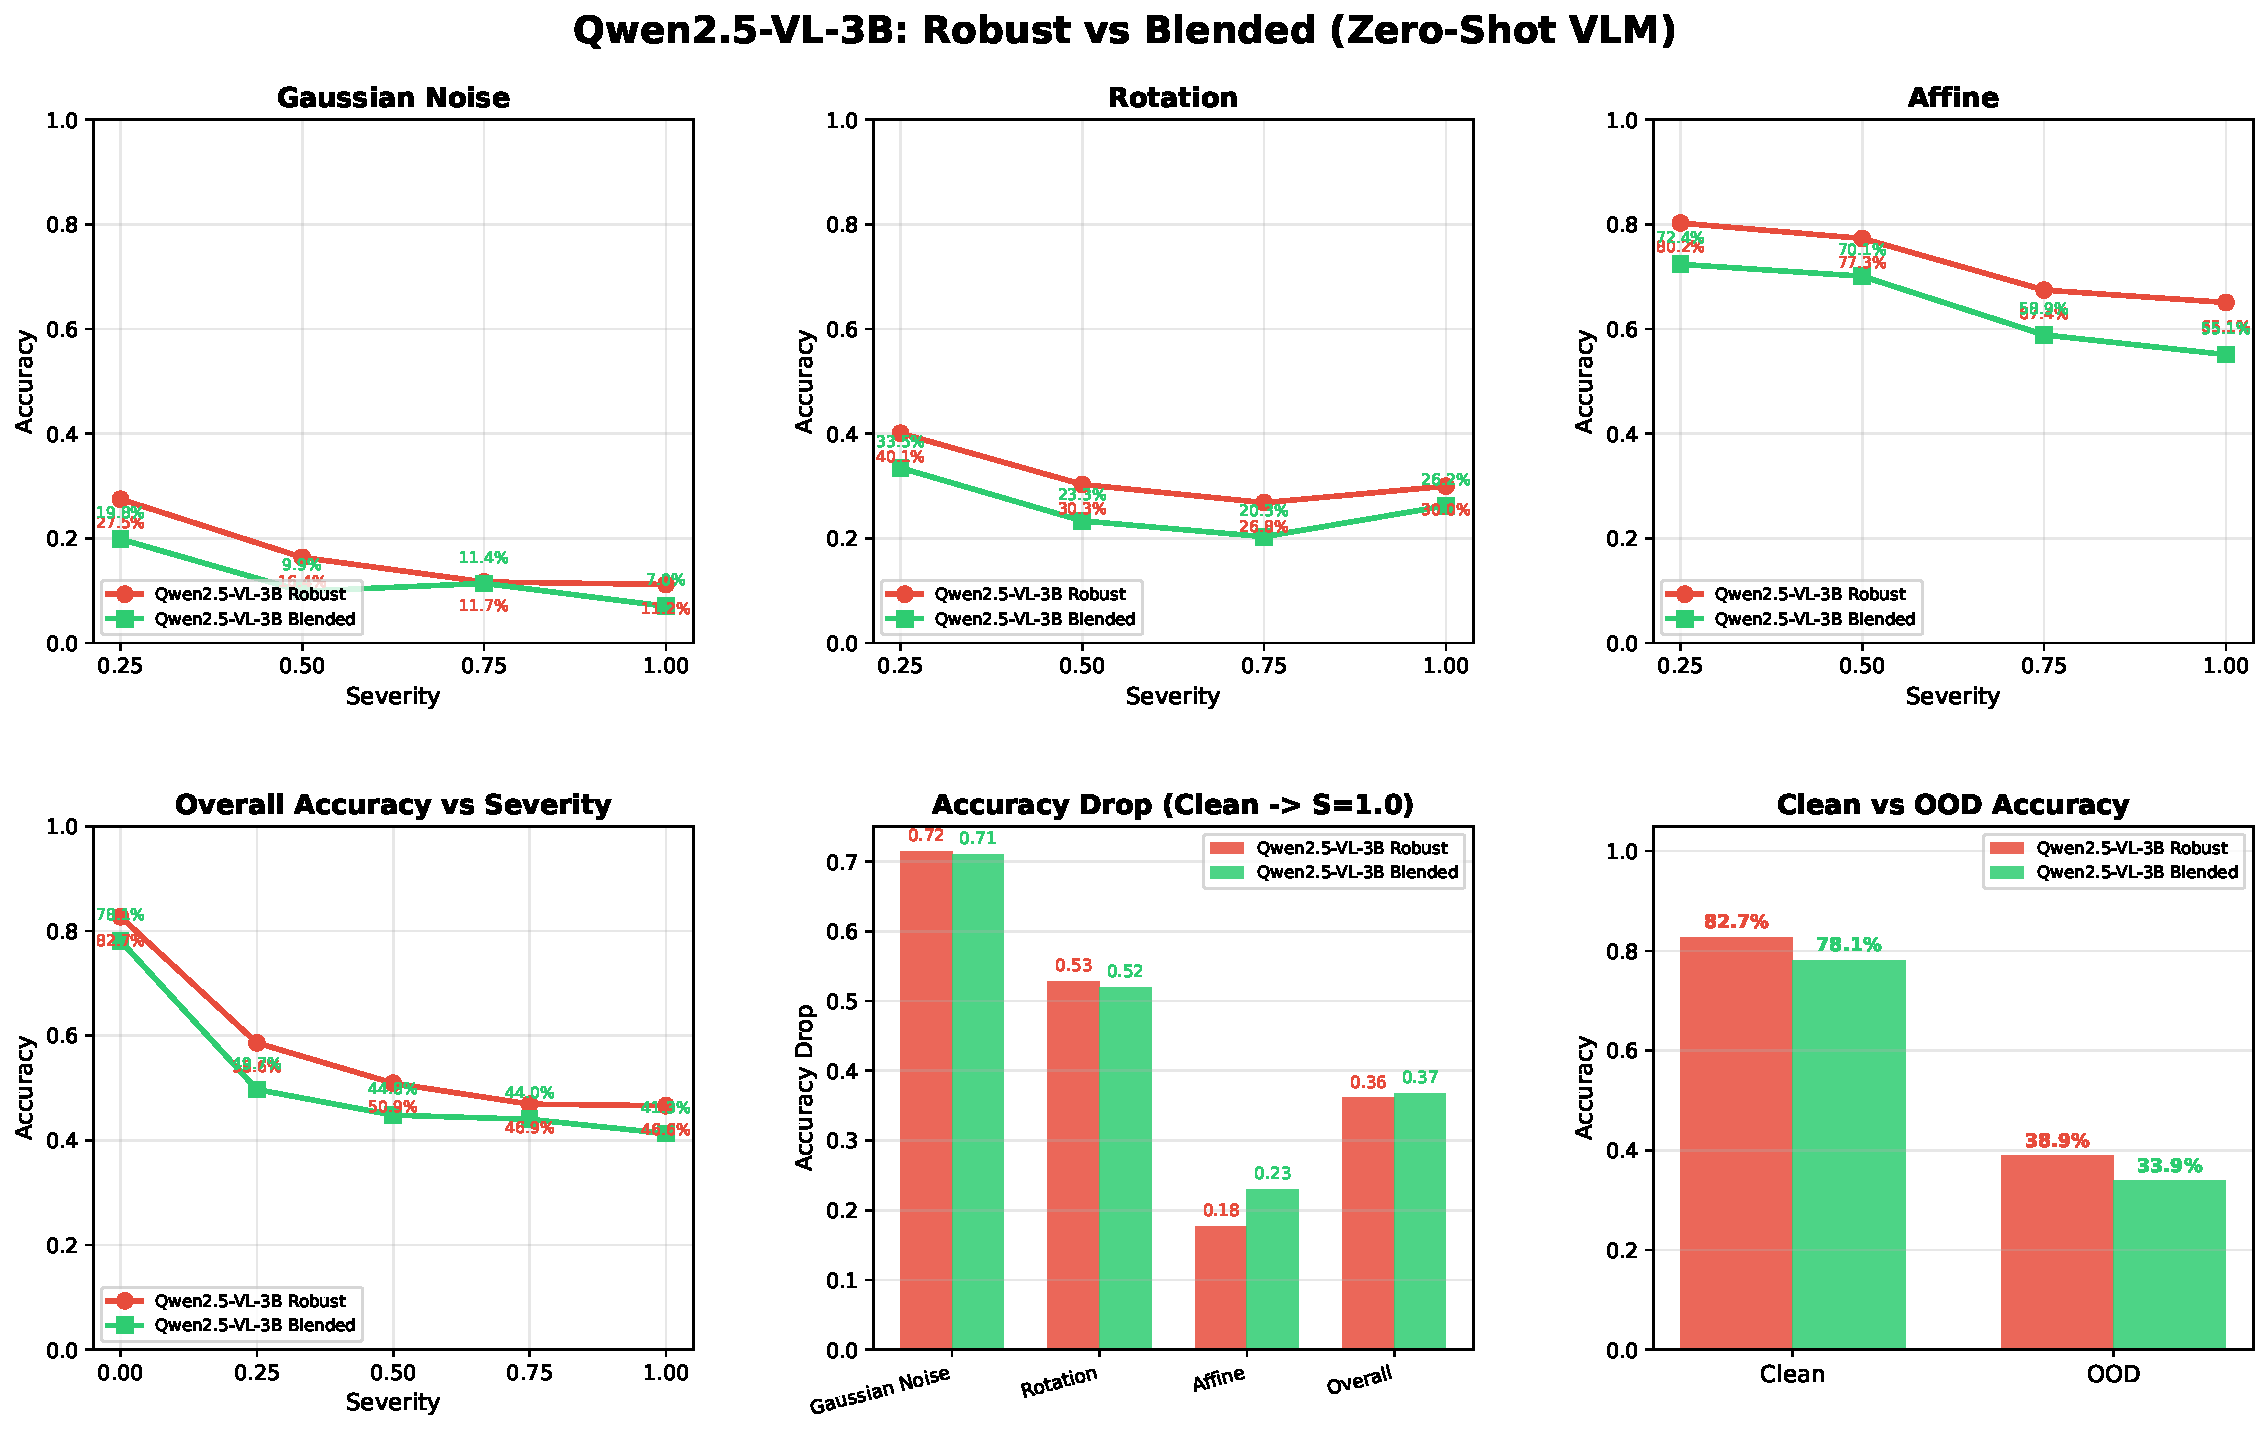
\includegraphics[width=0.95\textwidth]{graphs/pair_qwen_vlm_robust_vs_blended.pdf}
\caption{Qwen2.5-VL-3B: Robust vs Blended zero-shot prompting comparison.}
\end{figure}

\end{document}